\documentclass{article}
\usepackage{ismir,amsmath,cite}
\usepackage{graphicx}
\usepackage{color}
\usepackage{subcaption}
\usepackage{url}
\usepackage{booktabs}

\def\baselinestretch{0.97}

\title{Extracting Ground-Truth Information from MIDI Files:\\A MIDIfesto}

%\oneauthor
% {Colin Raffel and Daniel P. W. Ellis}
% {LabROSA \\ Department of Electrical Engineering \\ Columbia University \\ New York, NY}

\threeauthors
  {First Author} {Affiliation1 \\ {\tt author1@ismir.edu}}
  {Second Author} {\bf Retain these fake authors in\\\bf submission to preserve the formatting}
  {Third Author} {Affiliation3 \\ {\tt author3@ismir.edu}}

%% To make customize author list in Creative Common license, uncomment and customize the next line
%  \def\authorname{Colin Raffel, Daniel P. W. Ellis}

\sloppy

\begin{document}

\maketitle

\begin{abstract}
MIDI files abound and provide a bounty of information for music informatics.
We enumerate the types of information available in MIDI files and describe the steps necessary for utilizing them.
We also quantify the reliability of this data by comparing it to human-annotated ground truth.
The results suggest that developing better methods to leverage information present in MIDI files will facilitate the creation of MIDI-derived ground-truth for audio content-based MIR.
\end{abstract}

\section{MIDI Files}\label{sec:introduction}

MIDI (Music Instrument Digital Interface) is a hardware and software standard for communicating musical events.
First proposed in 1983 \cite{international1983midi}, MIDI remains a highly pervasive standard both for storing musical scores and communicating information between digital music devices.
Its use is perhaps in spite of its crudeness, which has been lamented since MIDI's early days \cite{moore1988dysfunctions}; most control values are quantized as 7-bit integers and information is transmitted at the relatively slow (by today's standards) 31,250 bits per second.
Nevertheless, its efficiency and well-designed specification make it a convenient way of formatting digital music information.

In the present work, we will focus on MIDI files, which in a simplistic view can be considered a compact way of storing a musical score.
MIDI files are specified by an extension to the MIDI standard \cite{international1988standard} and consist of a sequence of MIDI messages organized in a specific format.
A typical MIDI file contains timing and meter information in addition to a collection of one or more ``tracks'', each of which contains a sequence of notes and control messages.
The General MIDI standard further specifies a collection of 128 instruments on which the notes can be played, which standardizes the playback of MIDI files and has therefore been widely adopted.

When paired with a General MIDI synthesizer, MIDI files have been used as a sort of (highly lossy) perceptual audio codec, with entire songs only requiring a few kilobytes of storage.
The early availability of this ``coding method'', combined with the expense of digital storage in the 90s, made MIDI files a highly pervasive method of storing and playing back songs before the advent of the MP3.
Even after high-quality perceptual audio codecs were developed and storage prices plummeted, MIDI files remained in use in resource-scarce settings such as karaoke machines and cell phone ringtones.
As a result, there is an abundance of MIDI file transcriptions of music available today; through a large-scale web scrape, we obtained 176,141 MIDI files with unique MD5 checksums.  
Given their wide availability, we believe that MIDI files are underutilized in the Music Information Retrieval community.

In this paper, we start by outlining the various sources of information present in MIDI files and reference relevant works which utilize them in Section \ref{sec:information}.
In Section \ref{sec:utilizing}, we discuss the steps needed to leverage MIDI-derived information as ground truth for content-based MIR.
We then establish a baseline for the reliability of MIDI-derived ground truth by comparing it to handmade annotations in Section \ref{sec:measuring}.
Finally, in Section \ref{sec:discussion}, we argue that improving the process of extracting information from MIDI files is a viable path for creating large amounts of ground truth data for MIR.

\section{Information Available in MIDI Files}
\label{sec:information}

While various aspects of MIDI files have been used in MIR research, to our knowledge there has been no unified overview of the information they provide, nor a discussion of the availability and reliability of this information in MIDI transcriptions found ``in the wild''.
We therefore present an enumeration of the different information sources in a typical MIDI file and discuss their applicability to different MIR tasks.
Because not all MIDI files are created equal, we also computed statistics about the presence and quantity of each information source across our collection of 176,141 MIDI files; the results can be seen in Figure \ref{fig:statistics} and will be discussed in the following sections.

\begin{figure*}
    \centering
    \begin{subfigure}{.23\textwidth}
        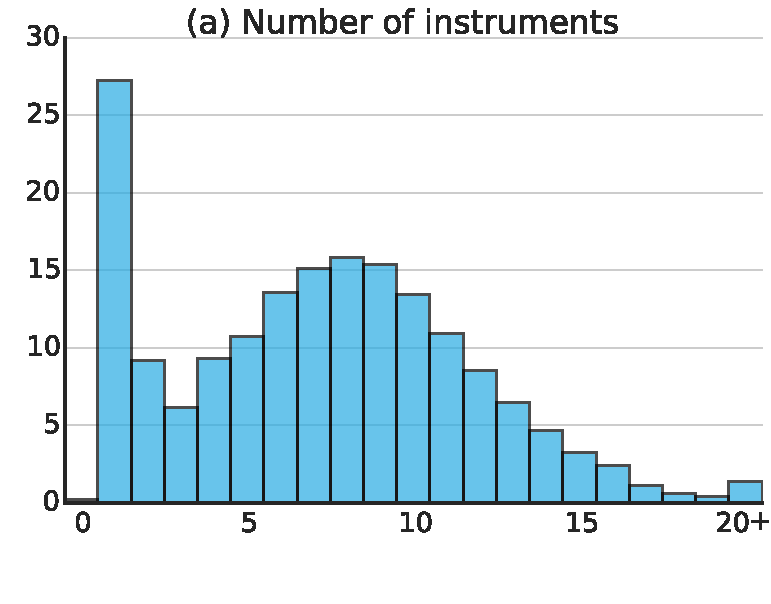
\includegraphics[width=\textwidth]{n_instruments.pdf}
    \end{subfigure}
    \begin{subfigure}{.23\textwidth}
        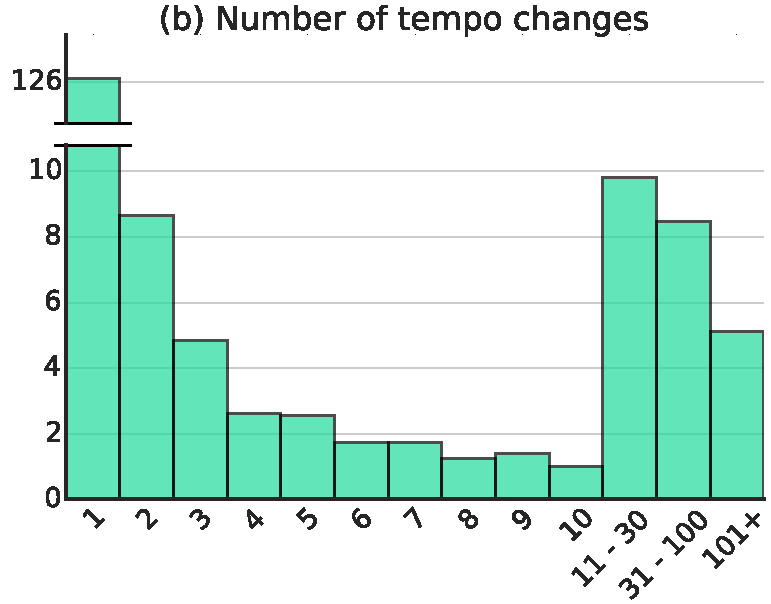
\includegraphics[width=\textwidth]{n_tempos.pdf}
    \end{subfigure}
    \begin{subfigure}{.23\textwidth}
        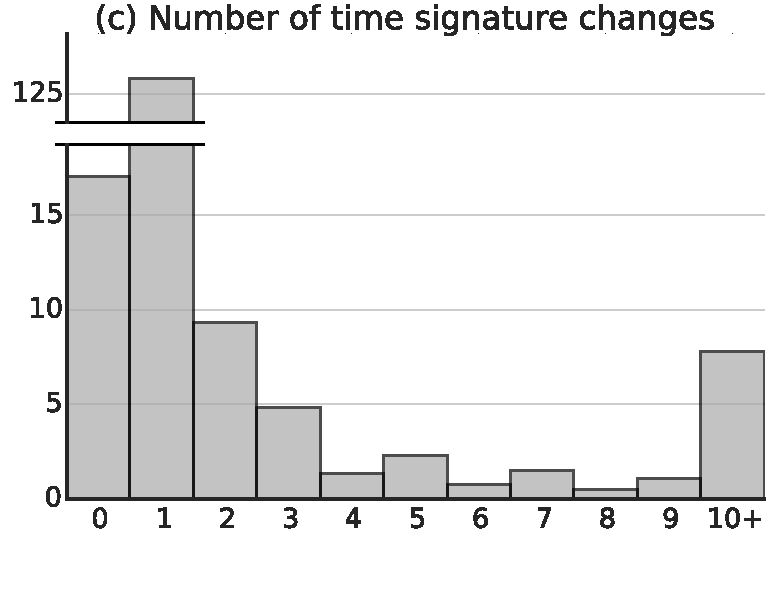
\includegraphics[width=\textwidth]{n_signatures.pdf}
    \end{subfigure}
    \begin{subfigure}{.23\textwidth}
        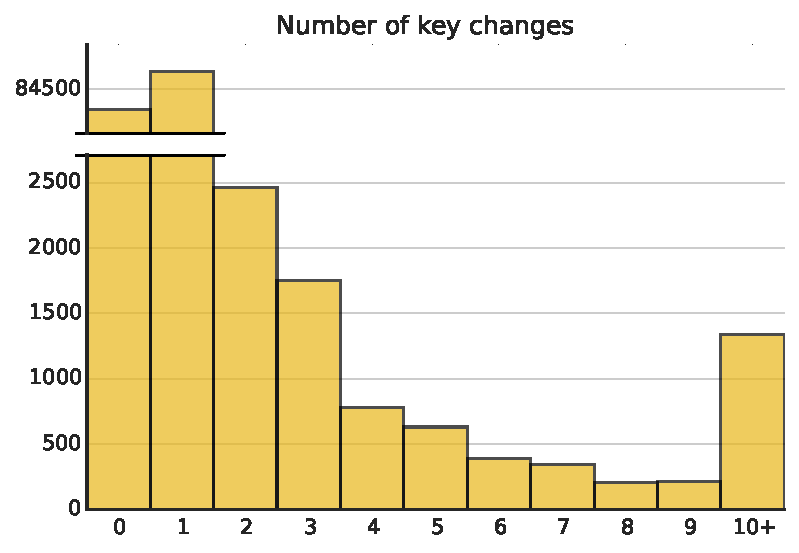
\includegraphics[width=\textwidth]{n_keys.pdf}
    \end{subfigure}

    \begin{subfigure}{.23\textwidth}
        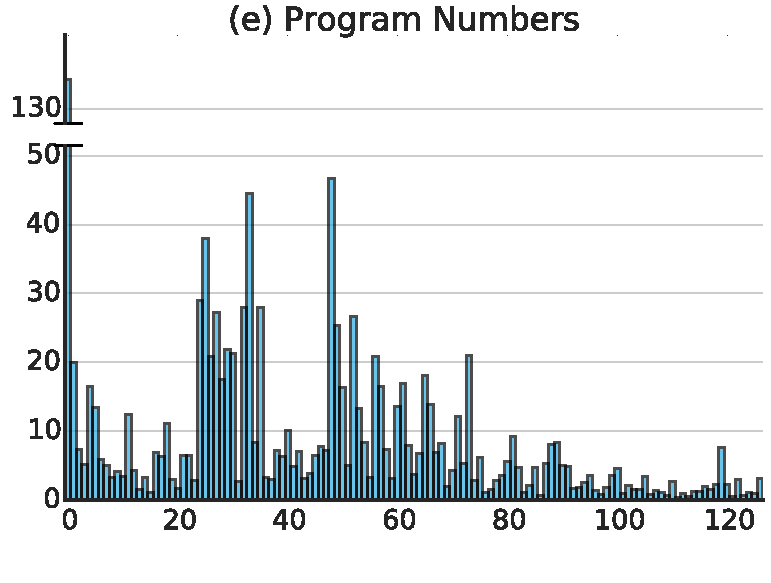
\includegraphics[width=\textwidth]{program_numbers.pdf}
    \end{subfigure}
    \begin{subfigure}{.23\textwidth}
        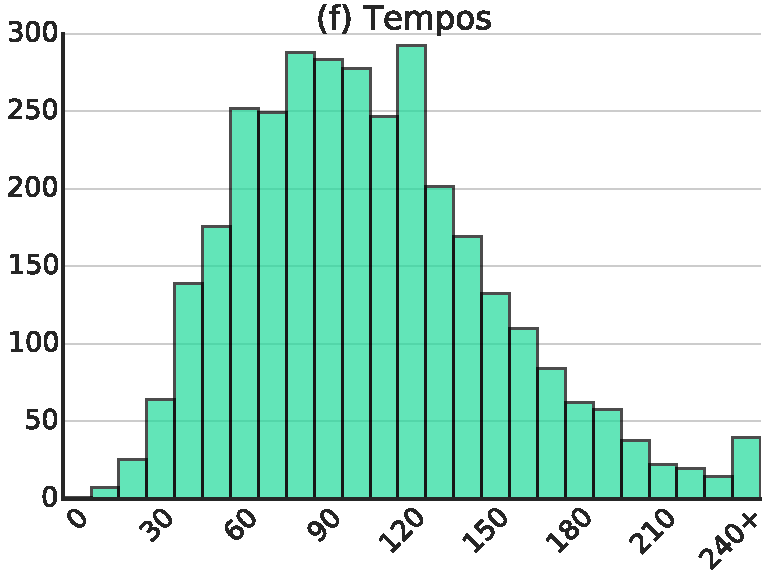
\includegraphics[width=\textwidth]{tempos.pdf}
    \end{subfigure}
    \begin{subfigure}{.23\textwidth}
        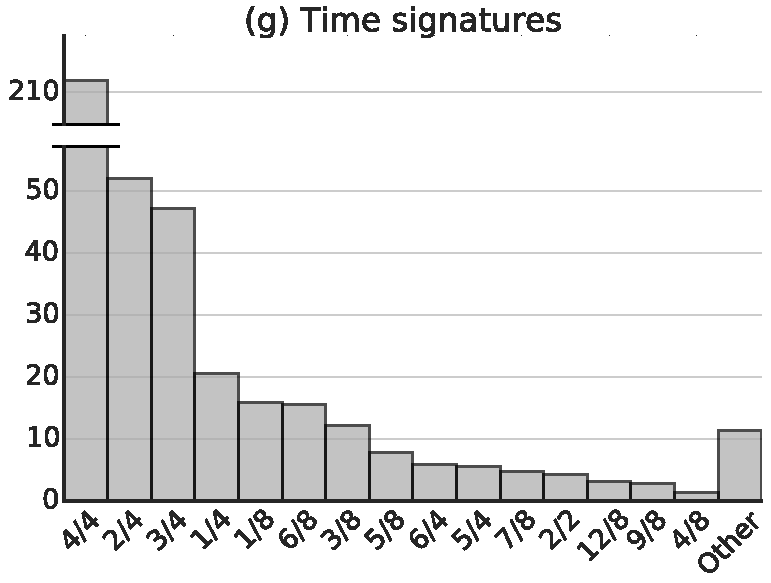
\includegraphics[width=\textwidth]{time_signatures.pdf}
    \end{subfigure}
    \begin{subfigure}{.23\textwidth}
        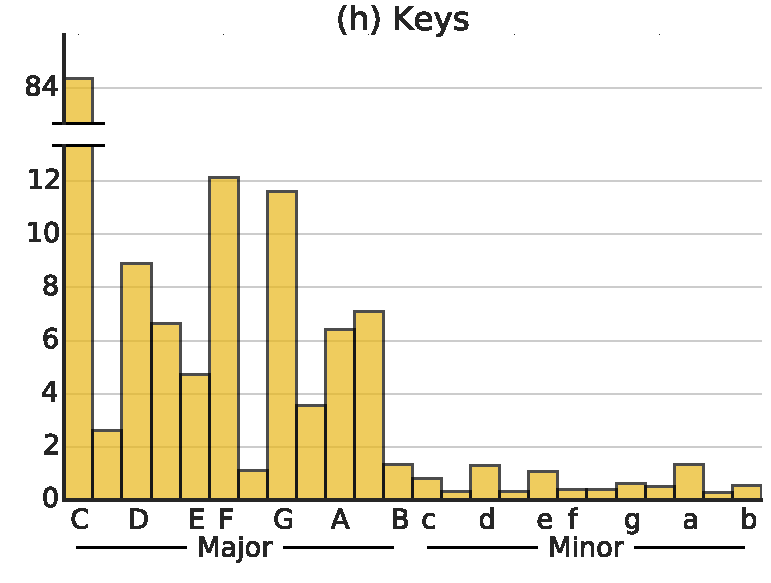
\includegraphics[width=\textwidth]{keys.pdf}
    \end{subfigure}
    \caption{Statistics about sources of information in 176,141 unique MIDI files scraped from the internet.
    Histograms in the top row show the number of MIDI files which had a given number of events for different event types; in the bottom row, we show distributions of the different values set by these events across all MIDI files.
    All counts are reported in thousands.
    For example, about 125,000 MIDI files had a single time signature change event, and about 210,000 4/4 time signature changes were found in all of our MIDI files.}
    \label{fig:statistics}
\end{figure*}

\subsection{Transcription}

MIDI files are specified as a collection of ``tracks'', where each track consists of a sequence of MIDI events on one of 16 channels.
Commonly used MIDI events are note on and note off messages, which together specify the start and end time of notes played at a given pitch on a given channel.
Various control events also exist, such as pitch bends, which allow for finer control of the playback of the MIDI file.
Program change events determine which instrument these events are sent to.
The General MIDI standard defines a correspondence between program numbers and a pre-defined list of 128 instruments.
General MIDI also specifies that all notes occurring on MIDI channel 10 play on a separate percussion instrument, which allows for drum tracks to be transcribed.
The distribution of the total number of program change events (corresponding to the number of instruments) across the MIDI files in our collection and the distribution of these program numbers are shown in Figures \ref{fig:statistics}(a) and \ref{fig:statistics}(e) respectively.
The four most common program numbers (shown as the four tallest bars in Figure \ref{fig:statistics}(e)) were 0 (``Acoustic Grand Piano''), 48 (``String Ensemble 1''), 33 (``Electric Bass (finger)''), and 25 (``Acoustic Guitar (steel)'').

This specification makes MIDI files naturally suited to be used as transcriptions of pieces of music, due to the fact that they can be considered a sequence of notes played on a collection of instruments.
As a result, many MIDI files are transcriptions and are thus commonly used as training data for automatic transcription systems (see \cite{turetsky2003ground} for an early example).
This type of data also benefits score-informed source separation methods, which utilize the score as a prior to improve source separation quality \cite{ewert2014score}.
An additional natural use of this information is for ``instrument activity detection'', i.e.\ determining when certain instruments are being played over the course of a piece of music.
Finally, the enumeration of note start times lends itself naturally to onset detection, and MIDI data has therefore been used for this task \cite{bello2005tutorial}.

\subsection{Musicological Features}

Because many MIDI files are transcriptions of music, they can also be used to compute high-level musicological characteristics of a given piece.
Towards this end, the software library \texttt{jSymbolic} \cite{mckay2006jsymbolic} includes functionality to extract a wide variety of features, including instrumentation, rhythm, and pitch statistics.
Similarly, \texttt{music21} \cite{cuthbert2010music21} provides a general-purpose framework for analyzing collections of digital scores (including MIDI files).
Computing these features on a collection of MIDI transcriptions is valuable for computational musicology and can enable data-driven corpus studies.
For example, \cite{cuthbert2011feature} discusses the use of \texttt{music21} and \texttt{jSymbolic} to extract features from scores and uses them to distinguish music from different composers and musical traditions.

\subsection{Meter}

Timing in MIDI files is determined by two factors: The MIDI file's specified ``resolution'' and tempo change events.
Each event within the MIDI file specifies the number of ``ticks'' between it and the preceding event.
The resolution, which is stored in the MIDI file's header, sets the number of ticks which correspond to a single beat.
The amount of time spanned by each tick is then determined according to the current tempo, as set by tempo change events.
For example, if a MIDI file has a resolution of 220 ticks per beat and the current tempo is 120 beats per minute,\footnote{Actually, tempo change events specify the number of microseconds per quarter beat, but this can be readily converted to beats per minute.} each tick would correspond to $60/(120*220) = 0.002\overline{27}$ seconds.
If a MIDI event in this file is specified to occur 330 ticks after the previous event, then it would occur $330*0.002\overline{27} = .75$ seconds later.

The timing in a MIDI file can vary over time by including many tempo change events.
In practice, as shown in Figure \ref{fig:statistics}(b), most MIDI files only contain a single tempo change and are therefore transcribed at a fixed tempo.
However, there are many MIDI files in our collection which have a large number of tempo change events (as indicated by the rightmost bars in Figure \ref{fig:statistics}(b)).
We have found that this is a common practice for making the timing of a MIDI transcription closely match that of an audio recording of the same song.
Despite the fact that the default tempo for a MIDI file is 120 beats per minute, Figure \ref{fig:statistics}(c) demonstrates that a wide range of tempos are used.
In practice, we find that this is due to the fact that even when a single tempo event is used, it is often set so that the MIDI transcription's tempo approximates that of an audio recording of the same song.

Time signature change events further augment MIDI files with the ability to specify time signatures, and are also used to indicate the start of a measure.
By convention, MIDI files have a time signature change at the first tick, although this is not a requirement.
Because time signature changes are relatively rare in western popular music, the vast majority of the MIDI files in our collection contain a single time signature change, as seen in Figure \ref{fig:statistics}(c).
Despite the fact that 4/4 is the default time signature for MIDI files and is pervasive in western popular music, a substantial portion (about half) included a non-4/4 time signature, as shown in Figure \ref{fig:statistics}(g).

Because MIDI files are required to include tempo information in order to specify their timing, it is straightforward to extract beat locations from a MIDI file.
By convention, the first (down)beat in a MIDI transcription occurs at the first tick.
Determining the beat locations in a MIDI file therefore involves computing beat locations starting from the first tick and adjusting the tempo and time signature according to any tempo change or time signature change events found.
Despite this capability, to our knowledge MIDI files have not been used as ground-truth for beat tracking algorithms.
However, \cite{mauch2012corpus} utilized a large dataset of MIDI files to study drum patterns using natural language processing techniques.


\subsection{Key}
\label{sec:key}

An additional useful event in MIDI files is the key change event.
Any of the 24 major or minor keys may be specified.
Key changes simply give a suggestion as to the tonal content and do not effect playback, and so are a completely optional meta-event.
As seen in Figure \ref{fig:statistics}(d), this results in many MIDI files omitting key change events altogether.
A further complication is that a disproportionate number (about half) of the MIDI files in our collection had key changes to the key of C major.
This disagrees with corpus studies of popular music, e.g.\ \cite{carlton2012analyzed} which found that only about 26\% of songs from the Billboard 100 were in C major.
We believe this is because many MIDI transcription software packages automatically insert a C major key change at the beginning of the file.

\subsection{Lyrics}

Lyrics can be added to MIDI transcriptions by the use of lyrics meta-events, which allow for timestamped text to be included over the course of the song.
This capability enables the common use of MIDI files for karaoke; in fact, a separate file extension ``.kar'' is often used for MIDI files which include lyrics meta-events.
Occasionally, the generic text meta-event is also used for lyrics, but this is not its intended use.
In our collection, we found 23,801 MIDI files (about 13.3\%) which had at least one lyrics meta-event.

\subsection{What's Missing}
\label{sec:missing}

Despite the wide variety of information sources available in MIDI files outlined in the previous sections, there are various types of information for which it is not possible (or not common) to store in MIDI files.
While the General MIDI specification includes the ``voice'' instruments ``Choir Aahs'', ``Voice Oohs'', ``Synth Choir'', ``Lead 6 (voice)'' and ``Pad 4 (choir)'', in practice there is no specific program number (or numbers) which is consistently used to transcribe vocals.
As a result, in a given MIDI file there is no reliable way of determining which instrument is a transcription of the vocals in a song.
Furthermore, because many MIDI files were designed for karaoke, the vocals may not be transcribed at all.

While the MIDI specification does include a ``track name'' meta-event, it is seldom used and there is no standard for its use, and so the instruments in MIDI files are further constrained to the General MIDI specification.
It follows that there is no simple way to retrieve the ``melody'' from a MIDI transcription, although the fact that all instruments are transcribed separately can make its estimation more straightforward than for audio files.
To our knowledge, there has been no research into automatically determining which instrument in a given MIDI file is a transcription of the melody or vocal line.

There is also no explicit way for MIDI files to include chord labels or structural segmentation boundaries (e.g.\ ``verse'', ``chorus'', ``solo'').
While this would in principle be possible thanks to the generic MIDI ``text'' meta-event, we have yet to find any MIDI files which store this information.
Nevertheless, estimating chords in particular is greatly facilitated by the presence of a ground-truth transcription.
Both \texttt{music21} \cite{cuthbert2010music21} and \texttt{melisma} \cite{sleator2001melisma} include functionality for estimating chord sequences from symbolic data.
Rhodes et al.\cite{rhodes2007bayesian} also proposed a symbolic chord estimation method using Bayesian Model Selection, which was shown to outperform \texttt{melisma} on a dataset of Beatles MIDI files in \cite{ewert2012towards}.

While text meta-events could also be used to store song-level metadata (song title, artist name, etc.) in a MIDI file, we have seldom encountered this in practice.
As a result, there is no standardized way to store this metadata in a MIDI file, although we found that a small portion of the filenames in our collection indicated the song title and occasionally the artist name.
The lack of a metadata specification also inhibits the attribution of MIDI transcriptions to the person who transcribed them.

\section{Utilizing MIDI Files as Ground Truth}
\label{sec:utilizing}

Utilizing MIDI files as ground-truth information for audio content-based MIR tasks requires the following:
First, the artist and song of a MIDI file must be determined and it must be matched to an audio recording of the song it is a transcription of.
Second, for many information sources, the MIDI file must be aligned in time with its matching audio recording.
Finally, the compact low-level binary format used by MIDI files must be parsed so that the information can be readily extracted.

\subsection{Matching}

Apart from metadata-agnostic corpus studies such as the one in \cite{mauch2012corpus}, determining what song a given MIDI file is is often a requirement.
Matching a given MIDI file to, for example, a corresponding entry in the Million Song Dataset \cite{bertin2011million} can be beneficial even in experiments solely involving symbolic data analysis because it can provide additional useful information about the MIDI file such as the song's year, genre, and user-applied tags.
Utilizing information in a MIDI file for ground-truth in audio content-based MIR tasks further requires that it be matched to an audio recording of the song.
Unfortunately, the lack of a standardized method for storing song-level metadata in MIDI files (as discussed in Section \ref{sec:missing}) complicates this necessity.
This has prompted the development of content-based matching methods; for example, early work by Hu et al.\cite{hu2003polyphonic} utilized the dynamic time warping (DTW) distance to compare spectrograms of MIDI syntheses and audio files and assigned matches by finding the minimal distance within the corpus.
This approach is prohibitively slow for very large collections of MIDI and/or audio files, so \cite{raffel2015large} explored learning a mapping from spectrograms to downsampled sequences of binary vectors, which greatly accelerates DTW.
\cite{raffel2016pruning} provided further speed-up by mapping entire spectrograms to fixed-length vectors in a Euclidean space where similar songs are mapped close together.
These methods make it feasible to quickly match a MIDI file to an extremely large corpus of audio recordings.

\subsection{Aligning}

There is no guarantee that a MIDI transcription for a given song was transcribed so that its timing matches an audio recording of a performance of the song.
For the many sources of ground-truth data which depend on timing (e.g.\ beats, transcription, or lyrics), the MIDI file must therefore have its timing adjusted so that it matches that of the performance.
Fortunately, there has been a great deal of research into score-to-audio alignment, and MIDI-to-audio alignment can be seen as a special ``offline'' case.
A highly common method is to use DTW or another edit-distance measure to find the best alignment between spectrograms of the synthesized MIDI and audio recording; see \cite{raffel2016optimizing} or \cite{ewert2012towards} for surveys.

In practice, audio-to-MIDI alignment systems can fail when there are overwhelming differences in timing or issues in the transcription, e.g.\ missing or incorrect instrumentation and/or notes.
Ideally, the alignment and matching processes could automatically report the success of the alignment and the quality of the MIDI transcription.
\cite{raffel2016optimizing} explores the ability of DTW-based alignment systems to automatically report a ``confidence'' score which denotes whether the alignment was successful or not.
To our knowledge, there has not been any research into automatically determining the quality of a MIDI transcription.

\subsection{Extracting Information}

The information sources enumerated in Section \ref{sec:information} are not readily available from MIDI files due to fact that they follow a low-level binary protocol.
For example, in order to extract the time (in seconds) of all onsets from a given instrument in a MIDI file, note events which occur on the same track and channel as program change events for the instrument must be collected and their timing must be computed from their relative ticks using the global tempo change events.
Fortunately, various software libraries have been created to facilitate this process.

The Python library \texttt{pretty\char`_midi} \cite{raffel2014pretty_midi} simplifies the extraction of useful information from MIDI transcriptions by taking care of most of the low-level parsing needed to convert the information to a more human-friendly format.
For example, it contains functions for retrieving beats, onsets, note lists from specific instruments, and the times and values of key, tempo, and time signature changes.
It also can be used to modify MIDI files, as well as to convert them to synthesized audio or a spectrogram-like piano roll representation.
The aforementioned Java library \texttt{jSymbolic} contains an extensive collection of routines for computing musicological features from MIDI files.
Finally, both \texttt{music21} and \texttt{melisma} are capable of inferring high-level music information from symbolic data of various types, including MIDI.

\section{Measuring a Baseline of Reliability for MIDI-Derived Information}
\label{sec:measuring}

Given the potential availability of ground-truth information in MIDI transcriptions, a natural question is the reliability of this data in MIDI transcriptions found ``in the wild''.
A straightforward way to evaluate the quality of data derived from a MIDI transcription of a given song would be to compare it to hand-made annotations for the song.
Given a MIDI transcription and human-annotated ground truth data, we can extract corresponding information from the MIDI file and compare using the heuristic evaluation metrics commonly used in the Music Information Retrieval Evaluation eXchange (MIREX) \cite{downie2008music}.
We therefore leveraged the Isophonics Beatles annotations \cite{mauch2009omras2} as a source of ground-truth to compare against MIDI-derived information because MIDI transcriptions of these songs are readily available due to The Beatles' popularity.

Our choice in tasks depends on the overlap in sources of information in the Isophonics annotations and MIDI transcriptions.
Isophonics includes beat times, song-level key information, chord changes, and structural segmentation.
As noted in Section \ref{sec:information}, beat times and key changes may be included in MIDI files but there is no standard way to include chord change or structural segmentation information.
We therefore performed experiments to evaluate the quality of key labels and beat times available in MIDI files.
Fortuitously, these two experiments give us an insight into both song-level timing-agnostic information (key) and alignment-dependent timing-critical information (beat).

To carry out these experiments, we first manually identified 545 MIDI files from our collection which had filenames indicating that they were transcriptions of songs from the Isophonics Beatles collection.
Of the 180 songs in the Isophonics Beatles collection, we found MIDI transcriptions for all but 11.
The median number of MIDI transcriptions per song was 2; the song ``Eleanor Rigby'' had the most, with 14 unique transcriptions.

\subsection{Key Experiment}

In our first experiment, we evaluated the reliability of key change events in MIDI files.
We followed the MIREX methodology for comparing keys \cite{ehmann2016mirex}, which proceeds as follows:
Each song may only have a single key.
All keys must be either major or minor, e.g.\ ``C\# Major'' and ``E minor'' are allowed but ``D Mixolydian'' is not.
An estimated key is given a score of 1.0 when it exactly matches a ground-truth key, 0.5 when it is a perfect fifth above the ground-truth key, 0.3 when it is a relative major or minor, 0.2 when it is a parallel major or minor, and 0.0 otherwise.
We utilized \texttt{mir\char`_eval} \cite{raffel2014mir_eval} to compute this score.

The Isophonics annotations mostly follow this format, except that 21 songs contained multiple key annotations and 7 others contained non-major/minor keys.
To simplify evaluation, we discarded these songs, leaving 179 ground-truth key annotations.
Of our 545 Beatles MIDIs, 221 had no key change event and 5 had more than one, which we also omitted from evaluation.
This left 223 MIDI files for which we extracted key annotations and compared them to valid Isophonics annotations.
Because of the preponderance of C major key change events noted in Section \ref{sec:key}, we also separately evaluated MIDI-derived C Major and non-C major instances separately to see whether they were less reliable.

As a baseline, we also extracted keys using the QM Vamp Key Detector plugin \cite{cannam2015mirex} whose underlying algorithm is based on \cite{noland2007signal} which finds the key profile which best correlates with the chromagram of a given song.
This plugin achieved the highest score in MIREX 2013, and has been the only key detection algorithm submitted in 2014 and 2015.
This gives us a reasonable expectation for a good audio content-based key estimator; to determine the extent to which human annotators agree on ground-truth key labels, we also collected key labels for Beatles' songs from \texttt{whatkeyisitin.com}.
As with the Isophonics key annotations, some songs had multiple and/or modal key labels; we discarded these and ended up with 145 labels for songs in the Isophonics dataset.

\begin{table}
\begin{center}
\begin{tabular}{lrr}
  \toprule
  Source                     & Score & Comparisons \\
  \midrule
  MIDI, all keys             & 0.400 &         223 \\
  MIDI, C major only         & 0.167 &         146 \\
  MIDI, non-C major          & 0.842 &          77 \\
  QM Key Detector            & 0.687 &         151 \\
  \texttt{whatkeyisitin.com} & 0.857 &         145 \\
  \bottomrule
\end{tabular}
\end{center}
  \caption{Mean scores achieved, and the number of comparisons made, by different datasets compared to Isophonics Beatles key annotations.}
  \label{tab:key}
\end{table}

The mean scores resulting from comparing each dataset to the Isophonics annotations can be seen in Table \ref{tab:key}.
At first glance, the mean score of $0.4$ achieved by MIDI key change messages is depressing.
However, by omitting all MIDI files with C major key events (which achieved a mean score of $0.167$), the mean score jumps to $0.842$.
This is comparable to the human-to-human baseline, and is substantially higher than the algorithmically estimated score.
We therefore propose that \textit{non-C major} MIDI key change events are as reliable as hand-annotated labels, but that C major key annotations in MIDI files are effectively useless.

\subsection{Beat Experiment}

\begin{figure*}
    \centerline{
    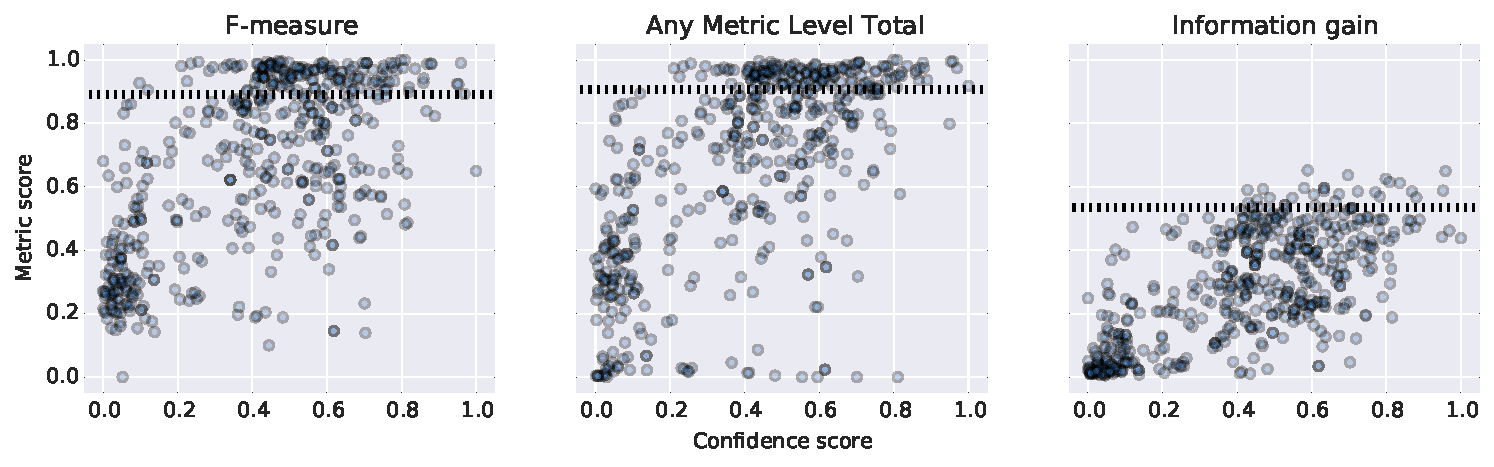
\includegraphics[width=\textwidth]{beat_scores.pdf}}
    \caption{Beat evaluation metric scores (compared to Isophonics beat annotations) and alignment confidence scores achieved by different audio-to-MIDI alignments of Beatles MIDI files, with each shown as a blue dot.
Mean scores for each metric achieved by the \texttt{DBNBeatTracker} \cite{bock2014multi} are shown as dashed lines.}
    \label{fig:beat}
\end{figure*}

Utilizing many of the sources of information in MIDI files in audio content-based MIR tasks depends on the precise alignment of a given MIDI file to an audio recording of a performance of the same song.
We therefore performed an additional experiment to evaluate the quality of MIDI-derived beat annotations, which are evaluated on the scale of tens of milliseconds.
Producing valid beat annotations from a MIDI file requires not only that the file's timing information is correct, but also that it has been aligned with high precision.

To align our Beatles MIDI files to corresponding audio recordings, we used the scheme proposed in \cite{raffel2016optimizing}, which was found by a large-scale search over common DTW-based audio-to-MIDI alignment systems.
We give an outline of this method below; for a full description, see \cite{raffel2016optimizing}.
First, the MIDI file is synthesized using the \texttt{fluidsynth} program.
Log-magnitude, constant-Q spectrograms of the synthesized MIDI and audio recording are extracted and their pairwise cosine distance matrix is computed.
The lowest-cost path through the distance matrix is then found using DTW, with the constraint that the path must span at least 96\% of the shorter of the two spectrograms.
In addition, all paths are penalized by adding the median value of the distance matrix each time a frame in one spectrogram is mapped to multiple frames in the other.
Finally, a ``confidence score'' is computed as the mean pairwise distance along the lowest-cost path, normalized by mean of the submatrix spanned by the path.

We followed \cite{raffel2016optimizing} exactly, except for the following changes:
First, instead of computing spectrograms with a hop size of 46 milliseconds, we used a hop of 23 milliseconds.
This finer timescale is more appropriate for the beat evaluation metrics we will use, which have tolerances measured in tens of milliseconds.
Second, the confidence scores computed using the method of \cite{raffel2016optimizing} lie in the range $[0.5, 1.0]$ where $0.5$ corresponds to ``highly confident'' and $1.0$ corresponds to ``likely wrong''; we re-scaled this range by subtracting $1$ and multiplying by $-2$, which results in the more easily interpretable range of $[0.0, 1.0]$ where higher scores mean higher confidence.

We used \texttt{pretty\char`_midi}'s \texttt{get\char`_beats} method to extract beat times from our 545 Beatles MIDI files, and adjusted each beat's timing according to the MIDI file's alignment to corresponding audio recordings.
For evaluation, we used the F-measure, Any Metric Level Continuous and Information Gain metrics described in \cite{davies2009evaluation}, as implemented in the evaluation library \texttt{mir\char`_eval} \cite{raffel2014mir_eval}.
As a baseline, we also computed beat locations using the \texttt{DBNBeatTracker} from the \texttt{madmom} software library,\footnote{\texttt{https://github.com/CPJKU/madmom}} which is based on the algorithm from \cite{bock2014multi}.
This represents a state-of-the-art general-purpose beat tracker which, on the Beatles data, can reliably produce high-quality annotations.
If MIDI-derived beat annotations are to be taken as ground truth, they must achieve scores similar to or higher than the \texttt{DBNBeatTracker}.

We visualize the resulting scores in Figure \ref{fig:beat}.
Because we don't expect beats to be extracted accurately from MIDI files which are poor transcriptions, we plotted each MIDI file as a single point whose x coordinate corresponds to the MIDI alignment confidence score and whose y coordinate is the resulting evaluation metric score achieved.
Ideally, all points in these plots would be clustered in the bottom left (corresponding to failed alignments with low confidence scores) or top right (corresponding to a successful alignment and beat annotation extraction with a high confidence score).
For reference, we plot the mean score achieved by the \texttt{DBNBeatTracker} as dotted lines for each metric.
From these plots, we can see that in many cases, MIDI ground truth achieves near-perfect scores, particularly for the F-Measure and Any Metric Level Continuous metrics.
However, there is no reliable correspondence between high confidence scores and high evaluation metric scores.
For example, while it appears that a prerequisite for an accurate MIDI-derived beat annotation is a confidence score above $.5$, there are many MIDI files which had high confidence scores but low metric scores (appearing in the bottom-right corner of the plots in Figure \ref{fig:beat}).

We found that this undesirable behavior was primarily caused by a few issues:
First, it is common that the alignment system would produce alignments which were slightly ``sloppy'', i.e.\ were off by one or two frames (corresponding to 23 milliseconds each) in places.
This had less of an effect on the F-measure and Any Metric Level Total metrics, which are invariant to small temporal errors up to a certain threshold, but deflated the Information Gain scores because this metric rewards consistent beat errors.
Second, many MIDI files had tempos which were at a different metric level than the annotations (e.g.\ double, half, or a third of the tempo).
This effected the Any Metric Level Total scores the least because it is invariant to these issues, except for the handful of files which were transcribed at a third of the tempo.
Finally, we found that the confidence score produced by the alignment system is most reliable at producing a low score in the event of a total failure (indicated by points in the bottom left of the plots in Figure \ref{fig:beat}), but was otherwise insensitive to the more minor issues that can cause beat evaluation metrics to produce low scores.

\section{Discussion}
\label{sec:discussion}

Our results suggest that while MIDI files have the potential to be valuable sources of ground-truth information, their usage may come with a variety of caveats.
However, due to the incredible number of MIDI transcriptions available, we submit that developing better methods to leverage information present in MIDI files is a tantalizing avenue for obtaining more ground-truth data for music information retrieval.
For example, while C-major key annotations cannot be trusted, developing a highly reliable C-major vs. non-C-major classification algorithm for symbolic data (which would ostensibly be much more tractable than creating a perfect general-purpose audio content-based key estimation algorithm) would enable the reliable usage of all key change messages in MIDI files.
Further work into robust audio-to-MIDI alignment is also warranted in order to leverage timing-critical information, as is the mostly neglected question of reliable alignment confidence score reporting.
Novel questions such as determining which MIDI instrument corresponds to the vocal or melody instrument in a given transcription, or determining whether all instruments have been transcribed, would also facilitate the use of MIDI files as ground-truth transcriptions.
Fortunately, all of these tasks are made easier by the fact that MIDI files are specified in a format from which it is straightforward to extract pitch information.
Any techniques developed towards this end could also be applied to other ubiquitous symbolic digital music formats such as MusicXML \cite{good2001musicxml}.

To facilitate further investigation, all 176,141 of the MIDI files we obtained in our web scrape (including our collection of 545 Beatles MIDIs) are available online,\footnote{\texttt{http://url-redacted.com}} as well as all of the code used in the experiments in this paper.\footnote{\texttt{http://url-redacted.com}}
We hope this data and discussion facilitates a groundswell of MIDI utilization in the MIR community.

\section{Acknowledgments}

We thank (redacted) % Eric J. Humphrey
and (redacted) % Hunter McCurry
for discussion about key evaluation and (redacted) % Rafael Valle
for investigations into MIDI beat tracking.

\small
\bibliography{refs}

\end{document}
